\chapter{KHẢO SÁT BÀI TOÁN VÀ THIẾT KẾ LƯỢC ĐỒ THỰC THỂ LIÊN KẾT (E-R)}

\section{Mô tả bài toán và Khảo sát yêu cầu}

\subsection{Bối cảnh và Quy mô hệ thống}
Trong khuôn khổ bài tập lớn môn học \textit{Các hệ thống Cơ sở dữ liệu}, đề tài đặt ra yêu cầu xây dựng một hệ thống cơ sở dữ liệu (CSDL) quản lý toàn diện một giải bóng đá chuyên nghiệp cấp quốc gia trong một mùa giải. Hệ thống phải đảm bảo theo dõi chặt chẽ tất cả các khía cạnh nghiệp vụ từ thông tin các câu lạc bộ, cầu thủ, sân vận động, đội ngũ trọng tài, cho đến công tác lập lịch thi đấu vòng tròn hai lượt, đăng ký đội hình trước trận đấu, diễn biến chi tiết sự kiện trên sân (bàn thắng, thẻ phạt) và tính toán bảng xếp hạng tự động.

Theo yêu cầu của đề bài, các thông số cơ bản của mùa giải được xác định như sau:
\begin{itemize}
    \item \textbf{Số lượng đội bóng tham gia}: Chọn $N = 6$ đội bóng (thỏa mãn yêu cầu số chẵn tối thiểu $\ge 6$).
    \item \textbf{Thể thức thi đấu}: Vòng tròn 2 lượt (lượt đi sân nhà, lượt về sân khách). Với 6 đội, số vòng đấu là $2 \times (6 - 1) = 10$ vòng đấu. Mỗi vòng đấu diễn ra 3 trận đấu cùng một thời điểm giữa 3 cặp đấu.
    \item \textbf{Tổng số trận đấu trong cả mùa giải}: $10 \text{ vòng} \times 3 \text{ trận/vòng} = 30 \text{ trận đấu}$. Toàn bộ lịch thi đấu và kết quả của 30 trận này phải được nhập đầy đủ vào hệ thống.
\end{itemize}

\subsection{Các quy tắc nghiệp vụ cốt lõi}
Hệ thống phải tuân thủ nghiêm ngặt các ràng buộc nghiệp vụ thế giới thực được nêu trong đề cương bài toán:
\begin{enumerate}
    \item \textbf{Ràng buộc về Đội bóng, Sân nhà và Trang phục}:
    \begin{itemize}
        \item Mỗi đội bóng sở hữu đúng 1 sân nhà cố định. Tuy nhiên, một sân vận động có thể là sân nhà của một hoặc nhiều đội bóng khác nhau.
        \item Mỗi đội bóng phải đăng ký tối thiểu từ 2 màu áo thi đấu trở lên (ví dụ: áo sân nhà, áo sân khách, áo phụ).
        \item Một đội bóng được đăng ký tối đa 30 cầu thủ trong danh sách thi đấu mùa giải.
    \end{itemize}
    \item \textbf{Ràng buộc về Cầu thủ, Hợp đồng và Số áo}:
    \begin{itemize}
        \item Mỗi cầu thủ ký hợp đồng chuyên nghiệp với một đội bóng chủ quản. Cầu thủ có thể được đem cho một đội bóng khác mượn trong một khoảng thời gian nhất định.
        \item Tại mỗi thời điểm, mỗi cầu thủ chỉ được phép thi đấu cho duy nhất một đội bóng.
        \item Số áo thi đấu của cầu thủ bắt buộc phải nằm trong miền giá trị từ $1$ đến $35$.
        \item Trong cùng một đội bóng, các cầu thủ không được phép trùng số áo nhau; cầu thủ ở hai đội bóng khác nhau hoàn toàn có thể mang cùng số áo.
    \end{itemize}
    \item \textbf{Ràng buộc về Trọng tài và Phân công điều khiển}:
    \begin{itemize}
        \item Mỗi trận đấu bắt buộc phải có đủ tổ gồm 4 trọng tài làm nhiệm vụ: 1 trọng tài chính, 2 trọng tài biên và 1 trọng tài bàn.
        \item Trong cùng một vòng đấu, một trọng tài chỉ được phép điều khiển tối đa 1 trận đấu.
    \end{itemize}
    \item \textbf{Ràng buộc về Đăng ký thi đấu và Khớp kết quả trận}:
    \begin{itemize}
        \item Trận đấu có hai trạng thái: \textit{Chưa diễn ra} (lịch thi đấu tương lai) hoặc \textit{Đã kết thúc}. Nếu trận đấu đã kết thúc, ngày giờ thi đấu không được vượt quá thời gian hiện tại.
        \item Trong mỗi trận đấu, mỗi đội bóng chỉ được đăng ký tối đa 18 cầu thủ (gồm đội hình xuất phát và danh sách dự bị).
        \item Danh sách các sự kiện bàn thắng, thẻ vàng, thẻ đỏ của từng cầu thủ trong mỗi trận phải được lưu vết chi tiết theo từng phút.
        \item \textbf{Toàn vẹn kết quả}: Tổng số bàn thắng và tổng số thẻ phạt của các cầu thủ ghi nhận trong trận phải khớp chính xác với tỉ số chung cuộc và số thẻ của đội bóng đó trong trận.
    \end{itemize}
\end{enumerate}

\subsection{Các chức năng và Ứng dụng triển khai trên hệ CSDL}
Hệ CSDL được thiết kế nhằm đáp ứng đầy đủ các ứng dụng quản lý và khai thác dữ liệu sau:
\begin{itemize}
    \item \textbf{Ứng dụng Quản trị danh mục}: Thực hiện thêm, xóa, sửa, tìm kiếm thông tin về đội bóng, cầu thủ, trọng tài, sân vận động, hợp đồng chuyển nhượng/cho mượn.
    \item \textbf{Ứng dụng Bảng xếp hạng giải đấu}: Tự động tính toán điểm số (Thắng = 3, Hòa = 1, Thua = 0) và sắp xếp thứ tự bảng xếp hạng theo chuẩn quốc tế:
    $$\text{Điểm} \rightarrow \text{Hiệu số bàn thắng/thua} \rightarrow \text{Tổng bàn thắng} \rightarrow \text{Số trận thắng sân khách} \rightarrow \text{Số thẻ đỏ (ít hơn)} \rightarrow \text{Số thẻ vàng (ít hơn)}.$$
    \item \textbf{Ứng dụng Thống kê Vua phá lưới}: Truy vấn danh sách 10 cầu thủ có tổng số bàn thắng cao nhất giải.
    \item \textbf{Ứng dụng Tính lương trọng tài theo tháng}: Tính thù lao điều khiển trận đấu của trọng tài dựa trên biểu phí quy định: Trọng tài chính: $3.000.000$ VNĐ/trận; Trọng tài biên: $2.000.000$ VNĐ/trận; Trọng tài bàn: $1.000.000$ VNĐ/trận.
    \item \textbf{Ứng dụng Thống kê Doanh thu sân vận động}: Tính toán doanh thu bán vé từng sân theo công thức: $\text{Doanh thu} = \sum (\text{Số khán giả} \times \text{Giá vé mỗi trận})$.
    \item \textbf{Ứng dụng Báo cáo vòng đấu}: Hiển thị chi tiết kết quả, tỉ số và các sự kiện của từng vòng đấu bất kỳ.
\end{itemize}

---

\section{Từ điển dữ liệu hệ thống}
Hệ thống được thiết kế bao gồm 11 bảng dữ liệu, chuẩn hóa nhằm tối ưu hóa tính độc lập và toàn vẹn dữ liệu:

\subsection{Bảng SAN\_VAN\_DONG (Sân vận động)}
Lưu trữ thông tin các sân vận động phục vụ tổ chức thi đấu.
\begin{table}[H]
\centering
\small
\begin{tabular}{|l|l|l|p{6cm}|}
\hline
\textbf{Tên trường} & \textbf{Kiểu dữ liệu} & \textbf{Ràng buộc} & \textbf{Mô tả / Ý nghĩa} \\ \hline
\texttt{MaSan} & VARCHAR(10) & PRIMARY KEY & Mã định danh duy nhất của sân \\ \hline
\texttt{TenSan} & NVARCHAR(100) & NOT NULL, UNIQUE & Tên sân vận động \\ \hline
\texttt{DiaChi} & NVARCHAR(200) & NOT NULL & Địa chỉ / Thành phố đặt sân \\ \hline
\texttt{SucChua} & INT & NOT NULL, CHECK > 0 & Sức chứa tối đa khán giả \\ \hline
\end{tabular}
\caption{Từ điển dữ liệu bảng SAN\_VAN\_DONG}
\end{table}

\subsection{Bảng DOI\_BONG (Đội bóng)}
Lưu trữ thông tin các câu lạc bộ tham dự giải.
\begin{table}[H]
\centering
\small
\begin{tabular}{|l|l|l|p{6cm}|}
\hline
\textbf{Tên trường} & \textbf{Kiểu dữ liệu} & \textbf{Ràng buộc} & \textbf{Mô tả / Ý nghĩa} \\ \hline
\texttt{MaDoi} & VARCHAR(10) & PRIMARY KEY & Mã định danh duy nhất của đội bóng \\ \hline
\texttt{TenDoi} & NVARCHAR(100) & NOT NULL, UNIQUE & Tên câu lạc bộ bóng đá \\ \hline
\texttt{HLV} & NVARCHAR(100) & NOT NULL & Họ tên Huấn luyện viên trưởng \\ \hline
\texttt{MaSanNha} & VARCHAR(10) & FOREIGN KEY & Mã sân nhà cố định ($\rightarrow$ \texttt{SAN\_VAN\_DONG}) \\ \hline
\end{tabular}
\caption{Từ điển dữ liệu bảng DOI\_BONG}
\end{table}

\subsection{Bảng MAU\_AO\_DOI\_BONG (Màu áo thi đấu)}
Lưu trữ các màu áo đăng ký thi đấu của mỗi đội (tối thiểu 2 màu).
\begin{table}[H]
\centering
\small
\begin{tabular}{|l|l|l|p{6cm}|}
\hline
\textbf{Tên trường} & \textbf{Kiểu dữ liệu} & \textbf{Ràng buộc} & \textbf{Mô tả / Ý nghĩa} \\ \hline
\texttt{MaDoi} & VARCHAR(10) & PK, FK & Mã đội bóng ($\rightarrow$ \texttt{DOI\_BONG}) \\ \hline
\texttt{LoaiMauAo} & VARCHAR(20) & PRIMARY KEY & Loại trang phục (\texttt{'SanNha'}, \texttt{'SanKhach'}, \texttt{'Phu'}) \\ \hline
\texttt{MoTaMau} & NVARCHAR(50) & NOT NULL & Mô tả màu sắc (VD: Đỏ - Trắng, Xanh tím than) \\ \hline
\end{tabular}
\caption{Từ điển dữ liệu bảng MAU\_AO\_DOI\_BONG}
\end{table}

\subsection{Bảng CAU\_THU (Cầu thủ)}
Lưu trữ thông tin hồ sơ nhân thân của cầu thủ.
\begin{table}[H]
\centering
\small
\begin{tabular}{|l|l|l|p{6cm}|}
\hline
\textbf{Tên trường} & \textbf{Kiểu dữ liệu} & \textbf{Ràng buộc} & \textbf{Mô tả / Ý nghĩa} \\ \hline
\texttt{MaCauThu} & VARCHAR(10) & PRIMARY KEY & Mã định danh duy nhất của cầu thủ \\ \hline
\texttt{HoTen} & NVARCHAR(100) & NOT NULL & Họ và tên cầu thủ \\ \hline
\texttt{NgaySinh} & DATE & NOT NULL & Ngày tháng năm sinh \\ \hline
\texttt{ViTri} & VARCHAR(20) & NOT NULL & Vị trí thi đấu sở trường \\ \hline
\texttt{QuocTich} & NVARCHAR(50) & NOT NULL & Quốc tịch \\ \hline
\end{tabular}
\caption{Từ điển dữ liệu bảng CAU\_THU}
\end{table}

\subsection{Bảng HOP\_DONG\_CAU\_THU (Hợp đồng và Đội bóng thi đấu)}
Lưu trữ hợp đồng chuyên nghiệp, quản lý tình trạng thi đấu và cho mượn cầu thủ.
\begin{table}[H]
\centering
\small
\begin{tabular}{|l|l|l|p{6cm}|}
\hline
\textbf{Tên trường} & \textbf{Kiểu dữ liệu} & \textbf{Ràng buộc} & \textbf{Mô tả / Ý nghĩa} \\ \hline
\texttt{MaHD} & VARCHAR(10) & PRIMARY KEY & Mã hợp đồng thi đấu \\ \hline
\texttt{MaCauThu} & VARCHAR(10) & FOREIGN KEY & Mã cầu thủ ($\rightarrow$ \texttt{CAU\_THU}) \\ \hline
\texttt{MaDoiChuQuan} & VARCHAR(10) & FOREIGN KEY & Đội sở hữu hợp đồng ($\rightarrow$ \texttt{DOI\_BONG}) \\ \hline
\texttt{MaDoiHienTai} & VARCHAR(10) & FOREIGN KEY & Đội đang thi đấu ($\rightarrow$ \texttt{DOI\_BONG}) \\ \hline
\texttt{SoAo} & INT & NOT NULL, CHECK (1..35) & Số áo thi đấu tại đội bóng hiện tại \\ \hline
\texttt{NgayBatDau} & DATE & NOT NULL & Ngày hợp đồng có hiệu lực \\ \hline
\texttt{NgayKetThuc} & DATE & NOT NULL & Ngày hết hạn hợp đồng ($> \text{NgayBatDau}$) \\ \hline
\texttt{TrangThai} & VARCHAR(20) & NOT NULL & \texttt{'ChinhThuc'} hoặc \texttt{'ChoMuon'} \\ \hline
\texttt{MucLuong} & DECIMAL(15,2) & CHECK $\ge 0$ & Lương cơ bản hàng tháng \\ \hline
\end{tabular}
\caption{Từ điển dữ liệu bảng HOP\_DONG\_CAU\_THU}
\end{table}

\subsection{Bảng TRONG\_TAI (Trọng tài)}
Lưu trữ hồ sơ danh sách trọng tài tham gia điều hành giải đấu.
\begin{table}[H]
\centering
\small
\begin{tabular}{|l|l|l|p{6cm}|}
\hline
\textbf{Tên trường} & \textbf{Kiểu dữ liệu} & \textbf{Ràng buộc} & \textbf{Mô tả / Ý nghĩa} \\ \hline
\texttt{MaTrongTai} & VARCHAR(10) & PRIMARY KEY & Mã định danh trọng tài \\ \hline
\texttt{HoTen} & NVARCHAR(100) & NOT NULL & Họ và tên trọng tài \\ \hline
\texttt{NgaySinh} & DATE & NOT NULL & Ngày tháng năm sinh \\ \hline
\texttt{QueQuan} & NVARCHAR(100) & NOT NULL & Tỉnh thành quê quán \\ \hline
\texttt{CapBac} & NVARCHAR(50) & NOT NULL & Cấp bậc trọng tài (FIFA, Quốc gia) \\ \hline
\end{tabular}
\caption{Từ điển dữ liệu bảng TRONG\_TAI}
\end{table}

\subsection{Bảng VONG\_DAU (Vòng đấu)}
Quản lý danh mục các vòng thi đấu của giải ($10$ vòng).
\begin{table}[H]
\centering
\small
\begin{tabular}{|l|l|l|p{6cm}|}
\hline
\textbf{Tên trường} & \textbf{Kiểu dữ liệu} & \textbf{Ràng buộc} & \textbf{Mô tả / Ý nghĩa} \\ \hline
\texttt{MaVong} & INT & PRIMARY KEY & Mã vòng đấu (1 đến 10) \\ \hline
\texttt{TenVong} & NVARCHAR(50) & NOT NULL, UNIQUE & Tên hiển thị vòng đấu \\ \hline
\texttt{ThuTu} & INT & NOT NULL, UNIQUE & Thứ tự thi đấu \\ \hline
\end{tabular}
\caption{Từ điển dữ liệu bảng VONG\_DAU}
\end{table}

\subsection{Bảng TRAN\_DAU (Trận đấu)}
Quản lý thông tin chi tiết từng trận đấu trong khuôn khổ mùa giải.
\begin{table}[H]
\centering
\small
\begin{tabular}{|l|l|l|p{6cm}|}
\hline
\textbf{Tên trường} & \textbf{Kiểu dữ liệu} & \textbf{Ràng buộc} & \textbf{Mô tả / Ý nghĩa} \\ \hline
\texttt{MaTran} & VARCHAR(10) & PRIMARY KEY & Mã định danh trận đấu \\ \hline
\texttt{MaVong} & INT & FOREIGN KEY & Vòng đấu ($\rightarrow$ \texttt{VONG\_DAU}) \\ \hline
\texttt{MaDoiNha} & VARCHAR(10) & FOREIGN KEY & Đội chủ nhà ($\rightarrow$ \texttt{DOI\_BONG}) \\ \hline
\texttt{MaDoiKhach} & VARCHAR(10) & FOREIGN KEY & Đội khách ($\rightarrow$ \texttt{DOI\_BONG}) \\ \hline
\texttt{MaSan} & VARCHAR(10) & FOREIGN KEY & Sân thi đấu ($\rightarrow$ \texttt{SAN\_VAN\_DONG}) \\ \hline
\texttt{NgayGio} & DATETIME & NOT NULL & Thời điểm bắt đầu trận đấu \\ \hline
\texttt{GiaVe} & DECIMAL(12,2) & NOT NULL, CHECK $\ge 0$ & Giá vé vào sân của trận đấu \\ \hline
\texttt{SoKhach} & INT & CHECK $\ge 0$, DEFAULT 0 & Số lượng khán giả theo dõi \\ \hline
\texttt{BanThangNha} & INT & CHECK $\ge 0$, DEFAULT 0 & Bàn thắng đội chủ nhà \\ \hline
\texttt{BanThangKhach} & INT & CHECK $\ge 0$, DEFAULT 0 & Bàn thắng đội khách \\ \hline
\texttt{TheVangNha} & INT & CHECK $\ge 0$, DEFAULT 0 & Thẻ vàng đội nhà \\ \hline
\texttt{TheVangKhach} & INT & CHECK $\ge 0$, DEFAULT 0 & Thẻ vàng đội khách \\ \hline
\texttt{TheDoNha} & INT & CHECK $\ge 0$, DEFAULT 0 & Thẻ đỏ đội nhà \\ \hline
\texttt{TheDoKhach} & INT & CHECK $\ge 0$, DEFAULT 0 & Thẻ đỏ đội khách \\ \hline
\texttt{TrangThai} & VARCHAR(20) & NOT NULL & \texttt{'ChuaDienRa'} hoặc \texttt{'DaKetThuc'} \\ \hline
\end{tabular}
\caption{Từ điển dữ liệu bảng TRAN\_DAU}
\end{table}

\subsection{Bảng PHAN\_CONG\_TRONG\_TAI (Phân công trọng tài)}
Ghi nhận tổ 4 trọng tài điều hành mỗi trận đấu.
\begin{table}[H]
\centering
\small
\begin{tabular}{|l|l|l|p{6cm}|}
\hline
\textbf{Tên trường} & \textbf{Kiểu dữ liệu} & \textbf{Ràng buộc} & \textbf{Mô tả / Ý nghĩa} \\ \hline
\texttt{MaTran} & VARCHAR(10) & PK, FK & Trận đấu ($\rightarrow$ \texttt{TRAN\_DAU}) \\ \hline
\texttt{VaiTro} & VARCHAR(20) & PRIMARY KEY & Vai trò: \texttt{'Chinh'}, \texttt{'Bien1'}, \texttt{'Bien2'}, \texttt{'Ban'} \\ \hline
\texttt{MaTrongTai} & VARCHAR(10) & FOREIGN KEY & Trọng tài được phân công ($\rightarrow$ \texttt{TRONG\_TAI}) \\ \hline
\end{tabular}
\caption{Từ điển dữ liệu bảng PHAN\_CONG\_TRONG\_TAI}
\end{table}

\subsection{Bảng DANG\_KY\_THI\_DAU (Danh sách đăng ký trận)}
Lưu trữ danh sách tối đa 18 cầu thủ được đăng ký thi đấu của mỗi đội trong mỗi trận.
\begin{table}[H]
\centering
\small
\begin{tabular}{|l|l|l|p{6cm}|}
\hline
\textbf{Tên trường} & \textbf{Kiểu dữ liệu} & \textbf{Ràng buộc} & \textbf{Mô tả / Ý nghĩa} \\ \hline
\texttt{MaTran} & VARCHAR(10) & PK, FK & Trận đấu ($\rightarrow$ \texttt{TRAN\_DAU}) \\ \hline
\texttt{MaCauThu} & VARCHAR(10) & PK, FK & Cầu thủ tham gia ($\rightarrow$ \texttt{CAU\_THU}) \\ \hline
\texttt{MaDoi} & VARCHAR(10) & FOREIGN KEY & Đội bóng đăng ký ($\rightarrow$ \texttt{DOI\_BONG}) \\ \hline
\texttt{LoaiDangKy} & VARCHAR(20) & NOT NULL & \texttt{'ChinhThuc'} hoặc \texttt{'DuBi'} \\ \hline
\texttt{SoAoTran} & INT & NOT NULL, CHECK (1..35) & Số áo mặc trong trận \\ \hline
\end{tabular}
\caption{Từ điển dữ liệu bảng DANG\_KY\_THI\_DAU}
\end{table}

\subsection{Bảng SU\_KIEN\_TRAN\_DAU (Sự kiện diễn biến trận)}
Lưu trữ chi tiết các biến cố bàn thắng, thẻ phạt theo từng phút.
\begin{table}[H]
\centering
\small
\begin{tabular}{|l|l|l|p{6cm}|}
\hline
\textbf{Tên trường} & \textbf{Kiểu dữ liệu} & \textbf{Ràng buộc} & \textbf{Mô tả / Ý nghĩa} \\ \hline
\texttt{MaSuKien} & VARCHAR(15) & PRIMARY KEY & Mã định danh sự kiện \\ \hline
\texttt{MaTran} & VARCHAR(10) & FOREIGN KEY & Trận đấu diễn ra ($\rightarrow$ \texttt{TRAN\_DAU}) \\ \hline
\texttt{MaCauThu} & VARCHAR(10) & FOREIGN KEY & Cầu thủ ghi bàn / nhận thẻ ($\rightarrow$ \texttt{CAU\_THU}) \\ \hline
\texttt{MaDoi} & VARCHAR(10) & FOREIGN KEY & Đội bóng được ghi nhận ($\rightarrow$ \texttt{DOI\_BONG}) \\ \hline
\texttt{LoaiSuKien} & VARCHAR(20) & NOT NULL & \texttt{'BanThang'}, \texttt{'TheVang'}, \texttt{'TheDo'} \\ \hline
\texttt{PhutGhiNhan} & INT & NOT NULL, CHECK (1..120) & Phút diễn ra sự kiện \\ \hline
\end{tabular}
\caption{Từ điển dữ liệu bảng SU\_KIEN\_TRAN\_DAU}
\end{table}

---

\section{Thiết kế Lược đồ Thực thể Liên kết (E-R Diagram)}

\subsection{Xác định các tập thực thể và Thuộc tính}
Dựa trên phân tích yêu cầu nghiệp vụ, hệ thống gồm các tập thực thể:
\begin{itemize}
    \item \textbf{Tập thực thể mạnh}:
    \begin{itemize}
        \item \texttt{SAN\_VAN\_DONG}: Khóa chính là \underline{\texttt{MaSan}}.
        \item \texttt{DOI\_BONG}: Khóa chính là \underline{\texttt{MaDoi}}.
        \item \texttt{CAU\_THU}: Khóa chính là \underline{\texttt{MaCauThu}}.
        \item \texttt{TRONG\_TAI}: Khóa chính là \underline{\texttt{MaTrongTai}}.
        \item \texttt{VONG\_DAU}: Khóa chính là \underline{\texttt{MaVong}}.
    \end{itemize}
    \item \textbf{Tập thực thể yếu và Thực thể quan hệ}:
    \begin{itemize}
        \item \texttt{MAU\_AO\_DOI\_BONG}: Thực thể yếu phụ thuộc vào \texttt{DOI\_BONG}, khóa bộ phận là \underline{\texttt{LoaiMauAo}}.
        \item \texttt{HOP\_DONG\_CAU\_THU}: Thực thể quan hệ mô tả hợp đồng giữa cầu thủ và các đội bóng, khóa chính là \underline{\texttt{MaHD}}.
        \item \texttt{TRAN\_DAU}: Thực thể quan hệ mô tả cuộc đối đầu giữa đội nhà và đội khách trong khuôn khổ một vòng đấu, khóa chính là \underline{\texttt{MaTran}}.
        \item \texttt{PHAN\_CONG\_TRONG\_TAI}: Mối kết hợp $N-N$ giữa trận đấu và trọng tài, khóa chính tổ hợp là (\underline{\texttt{MaTran}}, \underline{\texttt{VaiTro}}).
        \item \texttt{DANG\_KY\_THI\_DAU}: Mối kết hợp $N-N$ giữa trận đấu và danh sách cầu thủ, khóa chính tổ hợp là (\underline{\texttt{MaTran}}, \underline{\texttt{MaCauThu}}).
        \item \texttt{SU\_KIEN\_TRAN\_DAU}: Thực thể quan hệ biến cố, khóa chính là \underline{\texttt{MaSuKien}}.
    \end{itemize}
\end{itemize}

\subsection{Các mối quan hệ và Bản số (Cardinality)}
\begin{itemize}
    \item \textbf{Mối kết hợp \textit{SanNha} (\texttt{SAN\_VAN\_DONG} - \texttt{DOI\_BONG})}:
    Quan hệ $1 - N$. Một sân vận động có thể là sân nhà của $0, 1$ hoặc nhiều đội bóng ($0..N$). Một đội bóng bắt buộc có đúng 1 sân nhà ($1..1$).
    \item \textbf{Mối kết hợp \textit{DangKyMauAo} (\texttt{DOI\_BONG} - \texttt{MAU\_AO\_DOI\_BONG})}:
    Quan hệ $1 - N$. Một đội bóng có từ 2 màu áo trở lên ($2..N$). Một bản ghi màu áo thuộc về duy nhất 1 đội ($1..1$).
    \item \textbf{Mối kết hợp \textit{LichDau} (\texttt{VONG\_DAU} - \texttt{TRAN\_DAU})}:
    Quan hệ $1 - N$. Một vòng đấu gồm nhiều trận đấu ($3$ trận đối với giải 6 đội). Một trận đấu thuộc đúng 1 vòng đấu ($1..1$).
    \item \textbf{Mối kết hợp \textit{ThiDau} (\texttt{DOI\_BONG} - \texttt{TRAN\_DAU})}:
    Mỗi trận đấu gắn liền với đúng 2 đội bóng qua hai vai trò: Đội nhà (\texttt{MaDoiNha}) và Đội khách (\texttt{MaDoiKhach}).
    \item \textbf{Mối kết hợp \textit{PhanCong} (\texttt{TRAN\_DAU} - \texttt{TRONG\_TAI})}:
    Quan hệ $N - N$. Một trận đấu có đúng 4 trọng tài tương ứng với 4 vai trò. Một trọng tài chỉ được tham gia tối đa 1 trận trong một vòng đấu.
    \item \textbf{Mối kết hợp \textit{DangKy} (\texttt{TRAN\_DAU} - \texttt{CAU\_THU})}:
    Quan hệ $N - N$. Mỗi trận đấu lưu danh sách tối đa 18 cầu thủ được đăng ký của mỗi đội.
    \item \textbf{Mối kết hợp \textit{PhatSinhSuKien} (\texttt{TRAN\_DAU} - \texttt{SU\_KIEN\_TRAN\_DAU})}:
    Quan hệ $1 - N$. Một trận đấu phát sinh $0, 1$ hoặc nhiều sự kiện bàn thắng, thẻ phạt.
\end{itemize}

\subsection{Mô hình trực quan Lược đồ E-R}
Hình~\ref{fig:er_diagram} thể hiện tổng thể Lược đồ thực thể liên kết (E-R Diagram) chi tiết của hệ thống quản lý giải bóng đá chuyên nghiệp:

\begin{figure}[H]
	\centering
	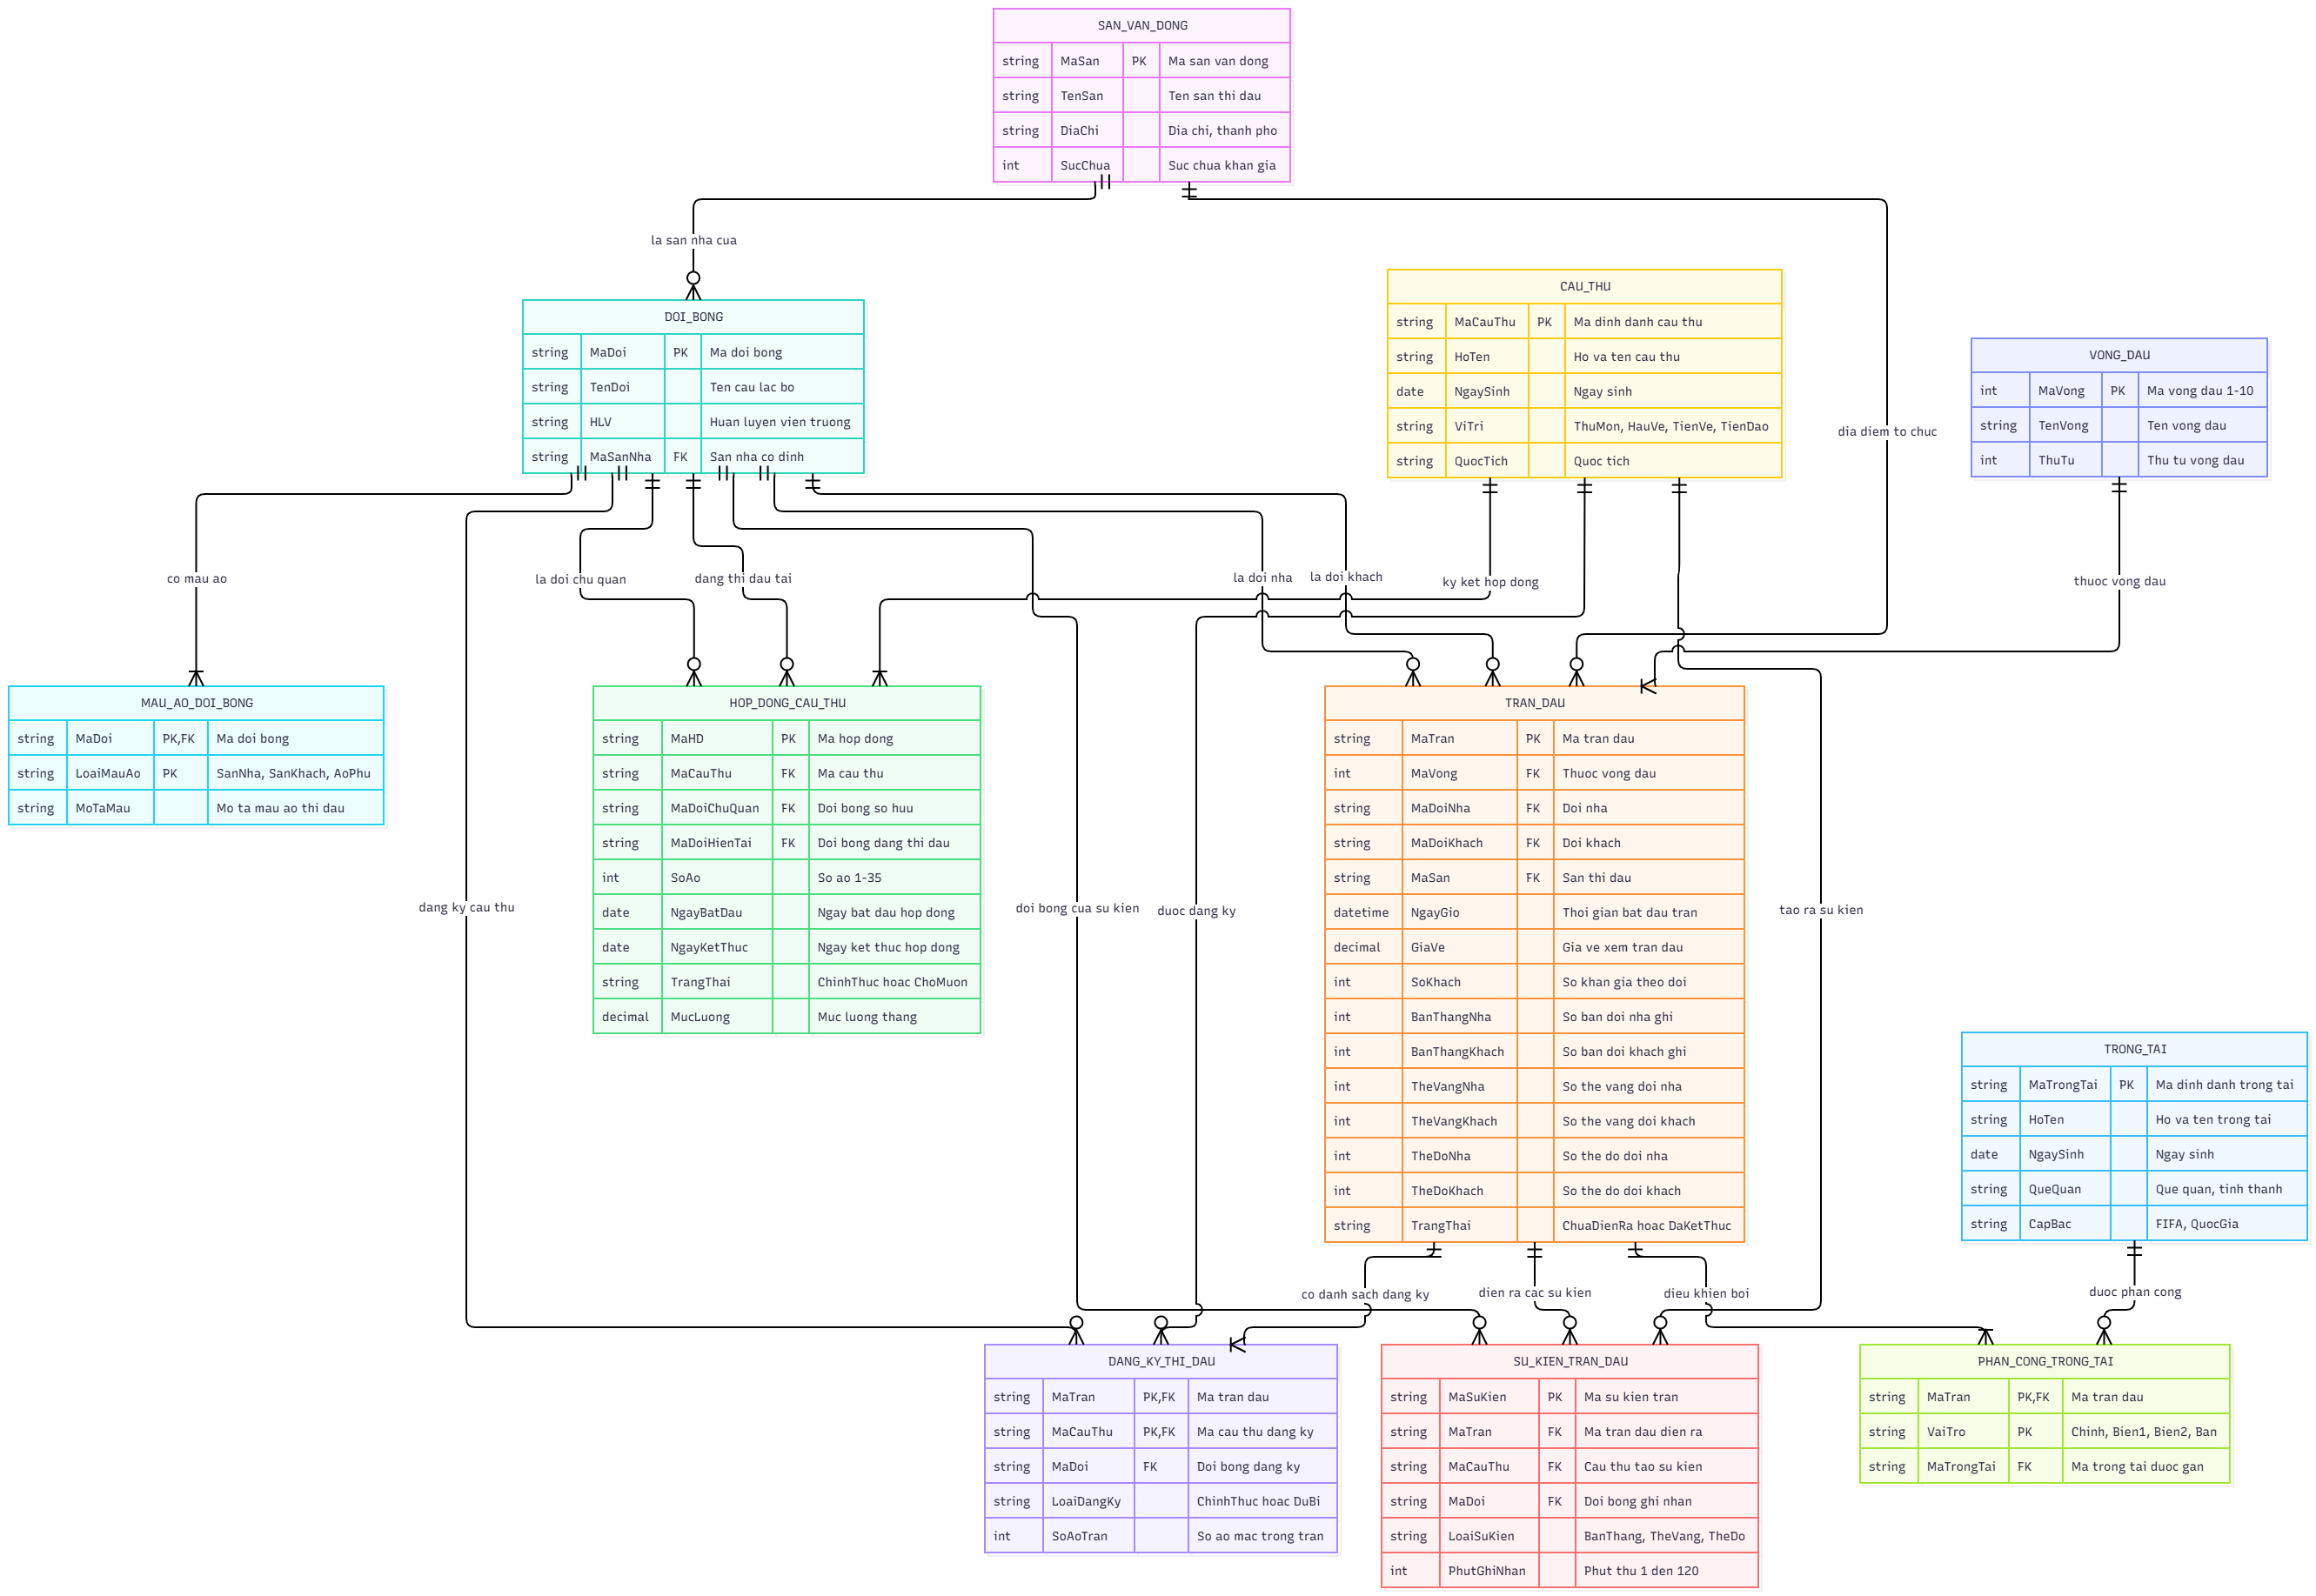
\includegraphics[width=\linewidth]{Figures/ERD.png}
    \caption{Sơ đồ cấu trúc lược đồ quan hệ và mối liên kết khóa}
    \label{fig:er_diagram}
\end{figure}
